\documentclass{article}

\usepackage{../preamble}
\standalonetrue

\title{MATH 316 Lecture 7}
\author{Ashtan Mistal}
\date{May 20 2021}

\begin{document}

\ifstandalone
\maketitle
\fi

\graphicspath{{./Lecture07/}}

\section{Boundary value Problems}

Is there a similar setup for BVPs/ Let's consider 3 different BVPs:
\begin{enumerate}
    \item P1: $y'' + \lambda y = 0$, for $x \in [0,L]$, with $y(0) = 0 = y(L)$
    \item P2: $y'' + \lambda y = 0$, for $x \in [0,L]$, with $y'(0) = 0 = y'(L)$
    \item P3: $y'' + \lambda y = 0$, for $x \in [0,L]$, with $y(0) = y(L)$ and $y'(0) = y'(L)$
\end{enumerate}

Any value of $\lambda$ for which P1 (P2 or P3) has a non-zero solution is called an \textbf{eigenvalue} of P1 (P2 or P3) and the corresponding solution is called and \textbf{eigenfunction} of P1 (P2 or P3).

Exercise: find the eigenvalues and eigenfunctions of problems P1, P2 and P3. 

\subsection{Solving BVP (P1,P2,P3)}

P1: \begin{center} $y'' + \lambda y = 0$, and $y(0) = 0 = y(L)$ \end{center}

$\lambda$: Eigenvalue. There are three categories that we have to investigate each time we solve such a problem:

\begin{enumerate}
    \item If $\lambda$ is negative ($\lambda < 0 $): 
    \begin{itemize}
        \item $\lambda = -\mu^2 \to y'' - \mu^2 y = 0$
        \item $r^2 - \mu^2 = 0 \to r_1 = \mu, r_2 = -\mu \longrightarrow y(x) = C_1 e^{\mu x} + C_2 e^{-\mu x}$
        \item Note that $\cosh(\mu x) = \frac{e^{\mu x} + e^{-\mu x}}{2} $ and $\sinh(\mu x) = \frac{e^{\mu x} - e^{-\mu x}}{2} \longrightarrow$
        \item $\hookrightarrow y(x) = A \sinh(\mu x) + B \cosh(\mu x)$
        \item 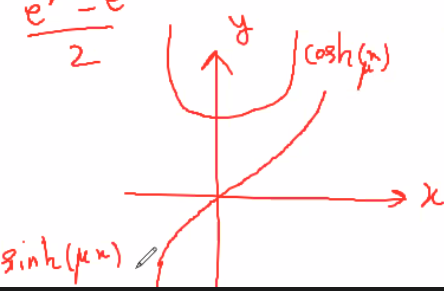
\includegraphics[width = 0.6 \textwidth]{image1.png}
        \item Note that we have the boundary conditions $y(0) = 0 \to B = 0$ and $y(L) = 0 \to A\sinh(\mu L) = 0$
        \item $\Rightarrow A = 0$ and $\Rightarrow y(x) = 0$ which is trivial
    \end{itemize}
    \item If $\lambda$ is zero: $y'' = 0 \longrightarrow y(x) = Ax + B$
    \begin{itemize}
        \item $y(0) = 0 \longrightarrow B = 0$
        \item $y(L) = 0 \longrightarrow AL = 0 \to A = 0 \to y(x) = 0$
        \item Therefore it's a trivial solution. 
    \end{itemize}
    \item If $\lambda > 0$: $\lambda = \mu^2 \to y'' + \mu^2 y = 0$
    \begin{itemize}
        \item $r^2 + \mu^2 = 0 \longrightarrow r = \pm i \mu$
        \item $y(x) = A \sin(\mu x) + B \cos(\mu x)$
        \item $y(0) = 0 \to B = 0$
        \item $y(L) = 0 \to A \sin(\mu L) = 0 \to \begin{matrix} A = 0 \text{(trivial)} \\ \sin(\mu L) = 0 \to \mu L = n \pi  \end{matrix} \text{ therefore } \mu = \frac{n \pi}{L}$
        \item Eigenvalue: $\lambda = \left(\frac{n \pi}{L} \right)^2$
        \item Eigenfunction: $y_n(x) = A_n \sin(\frac{n \pi}{L} x)$
    \end{itemize}
\end{enumerate}

\subsection{P2: $y'' + \lambda y = 0$}

$y'(0) = 0 = y'(L)$

$r^2 + \lambda = 0$
\begin{enumerate}
    \item If $\lambda > 0$, $\lambda = \mu^2$
    \begin{itemize}
        \item $r^2 + \mu^2 = 0 \longrightarrow r = \pm i \mu$
        \item $y(x) = A \sin(\mu x) + B \cos(\mu x)$
        \item Sub boundary conditions:
        \item $y'(0) = A = 0$ and $y'(L) = 0 \longrightarrow -B \mu \sin(\mu L) = 0$
        \item This gives us two solutions: $\begin{matrix} B = 0 \text{ which is trivial} \\ \underbrace{\sin(\mu L) = 0}_{\mu = \frac{n \pi}{L}} \end{matrix}$
        \item $\Rightarrow \lambda = \left( \frac{n \pi}{L}\right)^2$ is the eigenvalue
        \item $y_n (x) = B \cos \left( \frac{n \pi}{L} x \right)$ is the eigenfunction
        
    \end{itemize}
    \item If $\lambda < 0$: $\longrightarrow \lambda = -\mu^2$
    \begin{itemize}
        \item $r^2 - \mu^2 = 0 \longrightarrow r = \pm \mu \longrightarrow y(x) = C_1 e^{\mu x} + C_2 e^{-\mu x} \Rightarrow y(x) = A \sinh(\mu x) + B \cosh(\mu x)$
        \item Substituting the boundary conditions into $y(x) = A \sinh(\mu x) + B \cosh(\mu x)$, we get:
        \item $y'(0) = 0 \longrightarrow A = 0$
        \item $y'(L) = 0 \longrightarrow -\mu B \sinh (\mu L) = 0 \longrightarrow B = 0$ (which means that $y(x) = 0$ which is trivial)
    \end{itemize}
    \item If $\lambda = 0 \longrightarrow y'' = 0 \to y = Ax + B$
    \begin{itemize}
        \item $ y'(0) = 0 \to A = 0$ and $y'(L) = 0 \to A = 0$: $\longrightarrow$ $y(x) = B$
        \item $\lambda = 0$ is an eigenvalue $\longrightarrow y(x) = 1$ is the eigenfunction
        \item For P2 problems: eigenvalues are: $0, \frac{n^2 \pi^2}{L^2}$ and eigenfunctions are: $1, \cos\left(\frac{n \pi}{L} x \right)$
    \end{itemize}
\end{enumerate}

\subsection{P3: $y'' + \lambda y = 0$}

Periodic boundary conditions: $y(0) = y(L)$

\begin{enumerate}
    \item If $\lambda > 0$: $\lambda = \mu^2$
    \begin{itemize}
        \item $r = \pm \mu i \longrightarrow y(x) = A \sin(\mu x) + B \cos(\mu x)$
        \item $y(0) \ y(L) \longrightarrow B = A \sin(\mu L) + B \cos(\mu L)$
        \item $y'(0) = y'(L) \longrightarrow A \mu = A \mu \cos(\mu L) - B \mu \sin(\mu L)$
        \item 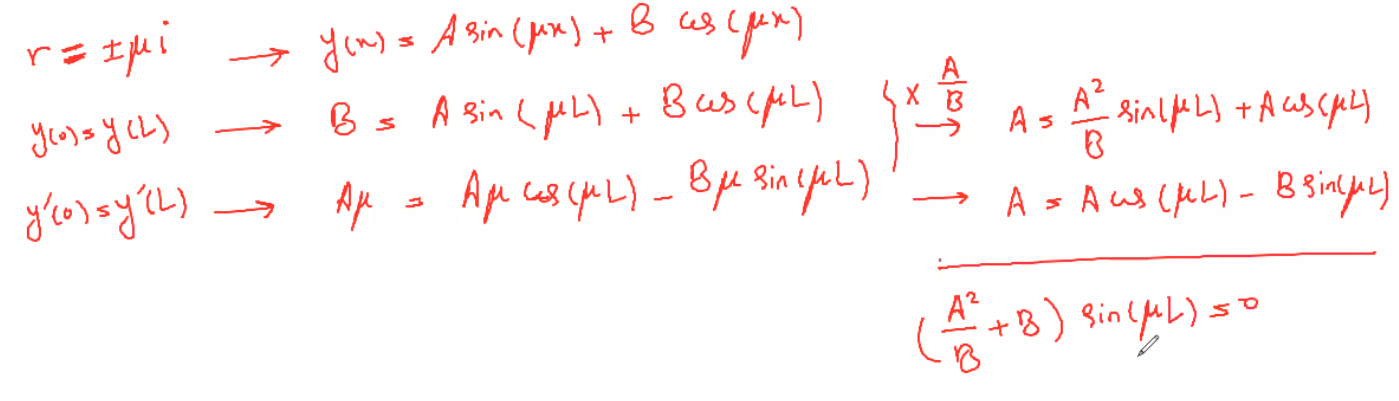
\includegraphics[width = 0.8 \textwidth]{image2.png}
        \item We get the last term by using the previous two terms (on the right) and cancelling out. 
        \item $\sin(\mu L) = 0 \to \mu L = n \pi$. $a \neq 0$ and $B \neq 0$ and therefore $\mu = \frac{n \pi}{L}$
        \item Eigenvalues: $\lambda = \left( \frac{n \pi}{L}\right)^2$
        \item Eigenfunction is $y_n (x) = A_n \sin(\frac{n \pi}{L} x) + B_n \cos(\frac{n \pi}{L} x)$
    \end{itemize}
    \item If $\lambda < 0$: $\lambda = -\mu^2$
    \begin{itemize}
        \item $y(x) = A \sinh(\mu x) + B \cosh(\mu x)$
        \item $y(0) = y(L) \longrightarrow B = A \sinh(\mu L) + B \cosh (\mu L)$
        \item $y'(0) = y'(L) \longrightarrow A = A \cosh(\mu L) - B \sinh(\mu L)$
        \item Multiplying $B = A \sinh(\mu L) + B \cosh (\mu L)$ by:
        \item 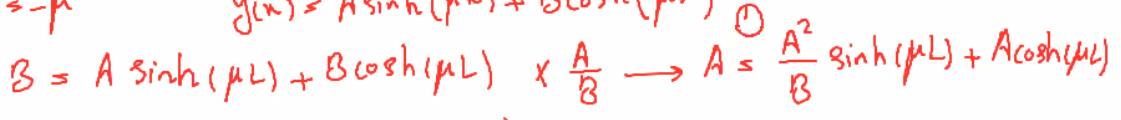
\includegraphics[width = 0.8 \textwidth]{image3.png}
        \item Okay this is going way too fast... screenshots it is. 
        \item 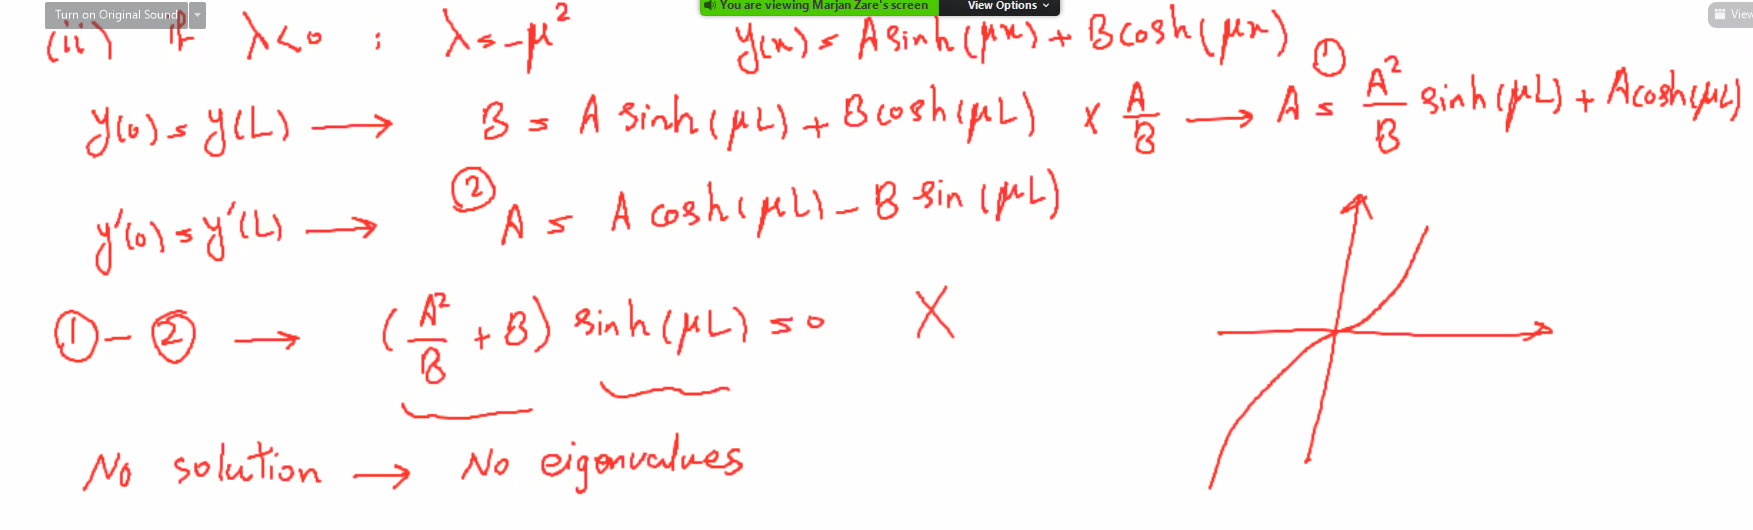
\includegraphics[width = 0.8 \textwidth]{image4.png}
    \end{itemize}
    \item $\lambda = 0$:
    \begin{itemize}
        \item View screenshot below. 
        \item 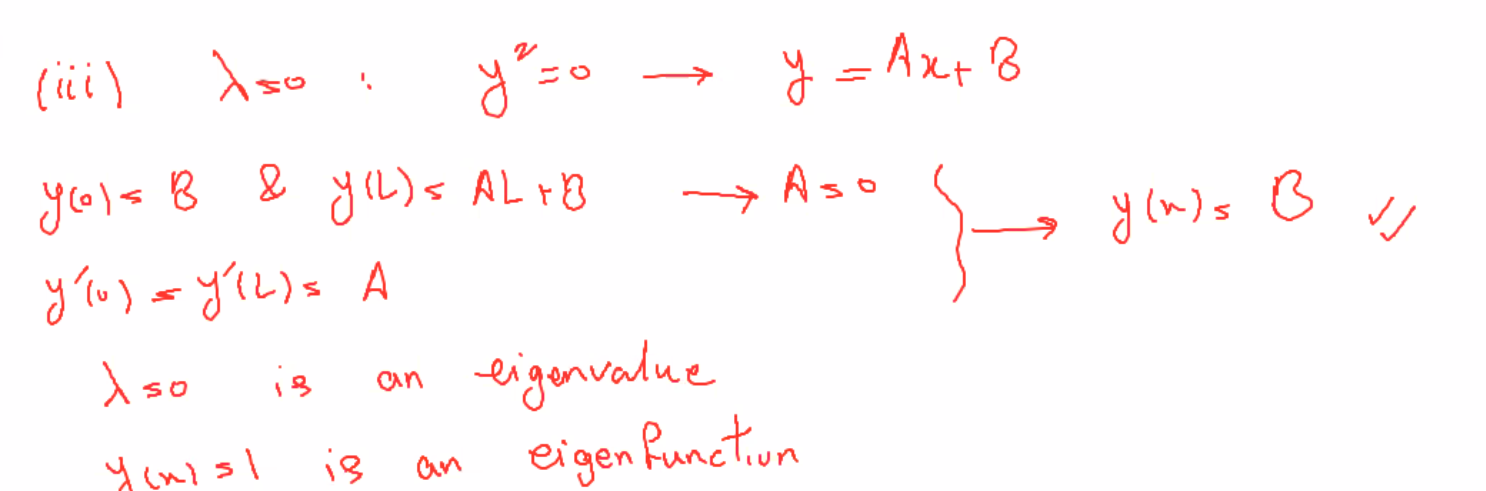
\includegraphics[width = 0.8 \textwidth]{image5.png}
    \end{itemize}
\end{enumerate}

\section{Fourier Series}

Fourier series arise in 3 different situations of relevance to this course:1.Simple boundary value problems, e.g. P1-P32.Partial differential equations that describe heat flow, waves and diffusion (more later).3.Some initial value problems with less simple periodic forcing, e.g. we are very unlikely to have exactly: $f(t) = F_0 \cos(\omega t)$, in any real system, but might have a periodic forcing function. \\ \hrule

\hfill

For what follows, let the interval in P1-P3 be the interval $[a,b] = [-L, L]$. The key idea is that an arbitrary function, $f(t)$, defined on $[-L, L]$ can be represented in the following form:

\begin{equation}
    f(t) = \frac{a_0}{2} + \sum_{n = 1}^\infty a_n \cos(\frac{n \pi t}{L}) + \sum_{n = 1}^\infty b_n \sin(\frac{n \pi t}{L})
\end{equation}

Note that these are the eigenfunctions of problem P3. Outside of the interval,because each function above has period $2L$, the above series must converge to a periodic extension of $f(t)$ of period $2L$.

Two immediate questions:
\begin{enumerate}
    \item Can all functions $f(t)$ be represented in this way, i.e. which functions?
    \item How do we find the coefficients $a_n$ and $b_n$?
\end{enumerate}

\textbf{Definition}:If the series on the right-hand side of (1) converges to a function $f(t)$ then this is called the Fourier series of $f(t)$. 

\hfill

Comments:

Firstly, in order for $f(t)$ to have Fourier series representation(1), that is valid for all $t$ it is necessary that $f(t)$ is periodic, with period $2L$, i.e. $$f(t + 2L) = f(t) \text{     } \forall t$$

Secondly, suppose that $f(t)$ has a Fourier series representation (1). Then $a_n$ and $b_n$ are determined straightforwardly. See below for $a_n$:

\begin{enumerate}
    \item Multiply (1) by $\cos(\frac{m \pi t}{L})$
    \item Integrate both sides of the equation between $[-L, L]$:
\end{enumerate}

$$\int_{-L}^{L} f(t) \cos \frac{m \pi t}{L} d t=\int_{-L}^{L}\left(\frac{a_{0}}{2}+\sum_{n=1}^{\infty} a_{n} \cos \frac{n \pi t}{L}+\sum_{n=1}^{\infty} b_{n} \sin \frac{n \pi t}{L}\right) \cos \frac{m \pi t}{L} d t$$

Note that:

$$
\begin{array}{l}
\int_{-L}^{L} \cos \frac{n \pi t}{L} \cos \frac{m \pi t}{L} d t=\left\{\begin{array}{ll}
0 & m \neq n \\
L & m=n
\end{array}\right. \\
\int_{-L}^{L} \cos \frac{n \pi t}{L} \sin \frac{m \pi t}{L} d t=0 \\
\int_{-L}^{L} \sin \frac{n \pi t}{L} \sin \frac{m \pi t}{L} d t=\left\{\begin{array}{ll}
0 & m \neq n \\
L & m=n
\end{array}\right.
\end{array}
$$

Therefore, interchanging summation and integration:

$$
\begin{aligned}
\int_{-L}^{L} f(t) \cos \frac{m \pi t}{L} d t &=a_{m} \int_{-L}^{L} \cos \frac{m \pi t}{L} \cos \frac{m \pi t}{L} d t=a_{m} L \\
a_{m} &=\frac{1}{L} \int_{-L}^{L} f(t) \cos \frac{m \pi t}{L} d t
\end{aligned}
$$

For the coefficients $b_n$ a similar procedure is possible (exercise). 

Thus, we finally have:

$$
\begin{aligned}
a_{0} &=\frac{1}{L} \int_{-L}^{L} f(t) d t \\
a_{m} &=\frac{1}{L} \int_{-L}^{L} f(t) \cos \frac{m \pi t}{L} d t \quad m=1,2,3, \ldots \\
b_{m} &=\frac{1}{L} \int_{-L}^{L} f(t) \sin \frac{m \pi t}{L} d t \quad m=1,2,3, \ldots
\end{aligned}
$$

which are known as the \textbf{Euler-Fourier series}. 

\subsection{Example 1}
\begin{center}
    Assumer that the function $f(t)$, defined by $(t) = \left\{ \begin{matrix} t & -L \leq t < 0 \\ 0 & 0 \leq t < L \end{matrix} \right.$ with $ f(t + 2L) = f(t)$, has a fourier series. Sketch the function and find the fourier series. 
\end{center}

Solution:

$$f(t) = \frac{a_0}{2} + \sum_{n = 1}^\infty a_n \cos(\frac{n \pi t}{L}) + \sum_{n = 1}^\infty b_n \sin(\frac{n \pi t}{L})$$

$$a_0 = \frac{1}{L} \int_{-L}^L f(t) dt = \frac{1}{L} \int_{-L}^0 t dt = \frac{-L}{2}$$

$$a_n = \frac{1}{L} \int_{-L}^L f(t) \cos(\frac{n \pi t}{L}) dt = \frac{1}{L} \int_{-L}^0 t \cos (\frac{n \pi t}{L}) dt$$. 

Using integration by parts, with $u = t$ ($du = dt$) and $dv = \cos(\frac{n \pi t}{L}) dt$, with $v = \frac{L}{n \pi} \sin(\frac{n \pi t}{L})$, we get the following:

$$a_n = \frac{1}{L} \left[\frac{tL}{n \pi} \frac{\sin(n \pi t)}{L} \right|_{-L}^0 - \int_{-L}^{0} \frac{L}{n \pi} \frac{\sin(n \pi t}{L} dt$$

$$ = \frac{1}{n \pi} \left[ \frac{L}{n \pi} \cos(\frac{n \pi t}{L} |_{-L}^{0} \right] = \frac{L}{n^2 \pi^2} \left(1 - \cos(n \pi \right)$$

\end{document}
